% This file was created by matlab2tikz.
%
\definecolor{mycolor1}{rgb}{0.00000,0.44700,0.74100}%
\definecolor{mycolor2}{rgb}{0.85000,0.32500,0.09800}%
\definecolor{mycolor3}{rgb}{0.92900,0.69400,0.12500}%
%
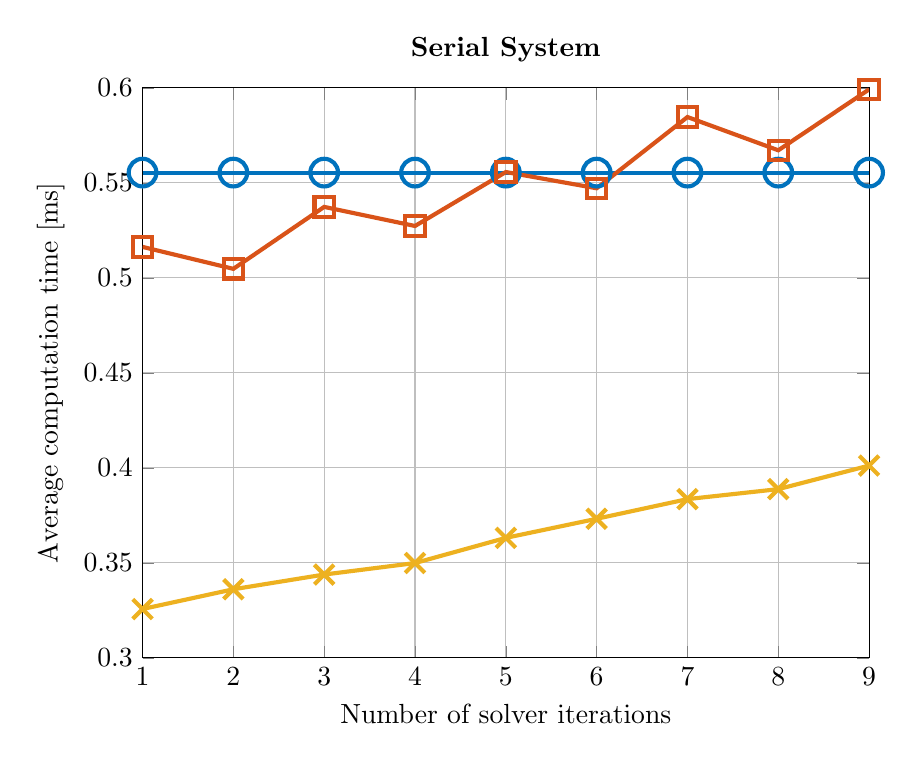
\begin{tikzpicture}

\begin{axis}[%
width=0.761\linewidth,
height=0.597\linewidth,
at={(0\linewidth,0\linewidth)},
scale only axis,
xmin=1,
xmax=9,
xlabel={Number of solver iterations},
xmajorgrids,
ymin=0.3,
ymax=0.6,
ylabel={Average computation time [ms]},
ymajorgrids,
axis background/.style={fill=white},
title style={font=\bfseries},
title={Serial System}
]
\addplot [color=mycolor1,solid,line width=1.5pt,mark size=5.0pt,mark=o,mark options={solid},forget plot]
  table[row sep=crcr]{%
1	0.5554\\
2	0.5554\\
3	0.5554\\
4	0.5554\\
5	0.5554\\
6	0.5554\\
7	0.5554\\
8	0.5554\\
9	0.5554\\
};
\addplot [color=mycolor2,solid,line width=1.5pt,mark size=3.5pt,mark=square,mark options={solid},forget plot]
  table[row sep=crcr]{%
1	0.5163\\
2	0.50475\\
3	0.53735\\
4	0.5273\\
5	0.5557\\
6	0.54715\\
7	0.58465\\
8	0.56715\\
9	0.5992\\
};
\addplot [color=mycolor3,solid,line width=1.5pt,mark size=5.0pt,mark=x,mark options={solid},forget plot]
  table[row sep=crcr]{%
1	0.3257\\
2	0.3361\\
3	0.34385\\
4	0.3499\\
5	0.36315\\
6	0.3732\\
7	0.38355\\
8	0.3888\\
9	0.4012\\
};
\end{axis}
\end{tikzpicture}%